\documentclass{article}
\usepackage[utf8]{inputenc}
\usepackage{hyperref}
\usepackage{enumitem}
\usepackage[english]{babel}
\usepackage{setspace}
\usepackage{lineno}
\usepackage[round]{natbib}
\usepackage{graphicx}
\usepackage{float}
\usepackage{amsmath}
\usepackage{amsthm}
\usepackage{amssymb}
\usepackage{bm}
\usepackage{subfig}
\usepackage{cleveref}
\usepackage{lipsum}
\usepackage{listings}



\title{Example \LaTeX{} Document}
\author{A. Uthor}
\date{\today}


\begin{document}

\maketitle

\newpage


\tableofcontents
\listoffigures
\listoftables

\newpage

\section{Introduction}\label{intro}
super and subscript: 10$^2$ 4$_f$ special characters: äáÈß\ss. A nice citation: \cite{hipsey_2019}.

There is a theory which states that if ever anyone discovers exactly what the Universe is for and why it is here, it will
instantly disappear and be replaced by something even more bizarre and inexplicable.
There is another theory which states that this has already happened  \citep{adams1995hitchhiker}.


\begin{figure}[t]
\centering
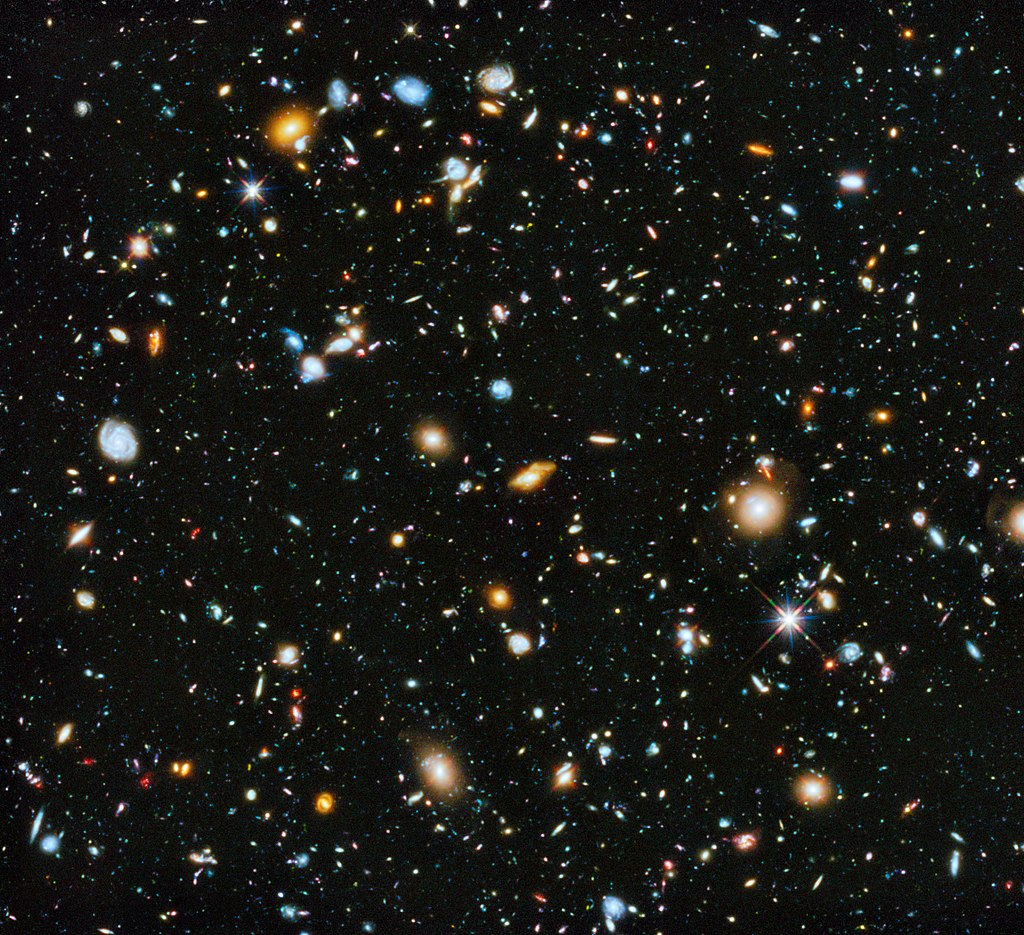
\includegraphics[width=0.5\linewidth]{universe.jpg}
\caption[The Universe]{The universe. Picture from NASA (\url{http://www.nasa.gov/hubble})}
\label{fig:galaxy}
\end{figure}

\section{Bullet points and numbering}

\begin{itemize}
    \item First Item
    \item Second item
    \item Another Item with numbered sub-items
    \begin{enumerate}
        \item Important stuff
        \item More important stuff
    \end{enumerate}
    \item And one last item
\end{itemize}

\section{Equations}

\subsection{Equation environments}
First equation using the equation environment:

\begin{equation}
y = a \cdot x + b
\end{equation}

Second equation using the align environment. This is useful for several equations that need to be aligned. The equations are aligned along the \& sign.

\begin{align}
y_1 &= a_{1,1} \cdot x_1 + a_{1,2} \cdot x_2 + b_1 \\
y_2 &= a_{2,1} \cdot x_1 + a_{2,2} \cdot x_2 + a_{2,3} \cdot x_3 b_2 + b_2 \\
y_3 &= a_{3,1} \cdot x_3 + b_3
\end{align}

\subsection{Equations in text}

A equation in running text $y = \frac{1}{x}$.

\section{Tables}

We can refer to \cref{tab:my_label} using the \texttt{\textbackslash{}cref\{key\}} command.

\begin{table}[b]
    \centering
    \caption[First table]{Caption of the table}
    \label{tab:my_label}
    \begin{tabular}{lll}\hline
        Name & ID & Value\\\hline
         Temp & 1  & 14  \\
         Temp & 2  & 16 \\
         Temp & 3 & 15 \\ \hline
    \end{tabular}
\end{table}

\section{Figures}

\subsection{One simple figure}
The milky way is the galaxy that contains our Solar System (\cref{fig:galaxy}).

\subsection{Multiple sub-figures}


\begin{figure}[t]%
    \centering
    \subfloat[The moon mission]{{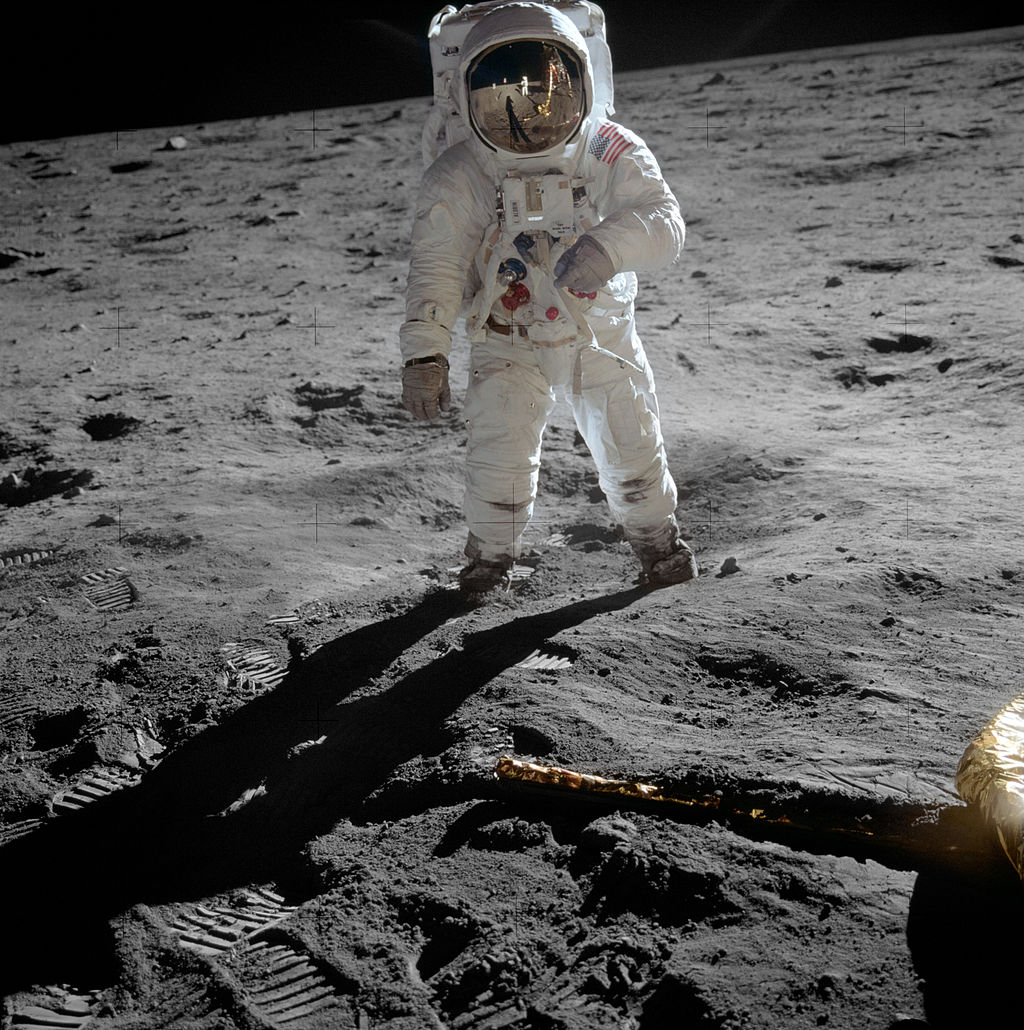
\includegraphics[width=5.5cm]{space-program-post.jpg} }}%
    \qquad
    \subfloat[International space station]{{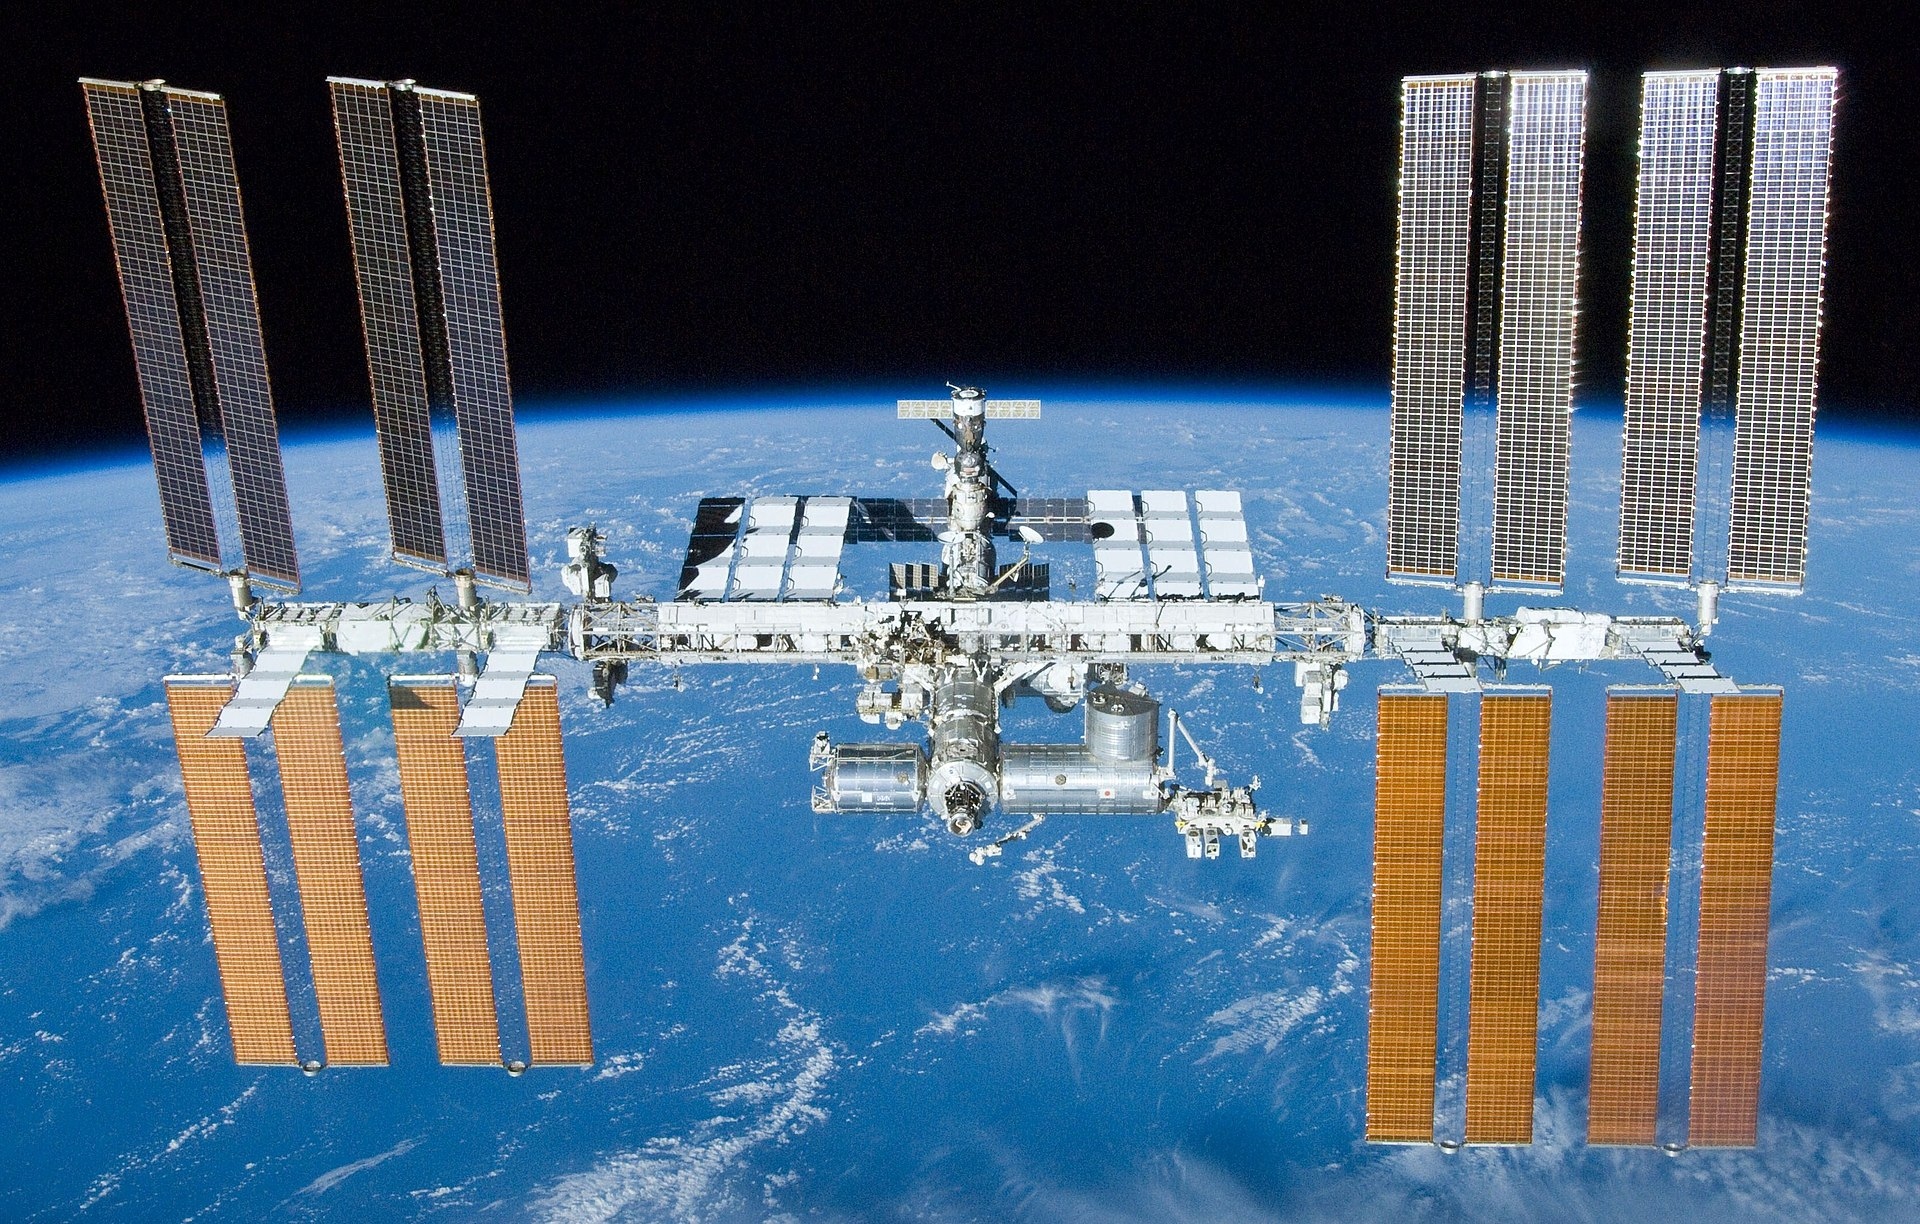
\includegraphics[width=5.5cm]{space-F.jpg} }}%
    \caption{Various space missions. Pictures from NASA.}%
    \label{fig:space}%
\end{figure}



In order to understand and unbox the mysteries of the universe as mentioned in \cref{intro}, scientists have launched various space programs (\cref{fig:space}).

\section{Tasks}

Please try to complete all given tasks. If you already have some experience try the advanced tasks in addition.

\subsection{Basic tasks:}

\begin{enumerate}
	\item Change the author name to your name
	\item Change the title of the document
    \item Include some of your own text
    \item Make some of your text bold and italics
    \item Change the fontsize of some of your text
    \item Include your favorite equation
    \item Include a figure you created
    \item Change the \textit{placement specifier} in a float and see what happens
    \item Change the alignment of one of your figures from centered to the left side
    \item Add your own table
    \item Refer to a (sub)section and the page it is on
    \item Add you own reference and cite them
    \item Try different style of referencing (Hint: use of different variations of command cite)
    \item add some formatted source code (Hint: use the lstlisting environment)
\end{enumerate}

\subsection{Advanced tasks:}

\begin{itemize}
    \item Change the used font
    \item Change the linespacing
    \item Add linenumbers
    \item Change the way equations are numbered so they start with the number of the section and then start counting by 1 in every section
    \item Change the symbol (point) in an \texttt{itemize} list
    \item Change the document to a two column format
    \item Add a table with customized text alignment in different columns and some combined columns
    \item Change the document from article style to any journal style of choice
    \item create a \LaTeX{} table from your own results using R (or python, or Matlab, or ...)
    \item Find your own Problem/idea and try to implement it
\end{itemize}

\bibliographystyle{abbrvnat}
\bibliography{references}
\end{document}
